\section{Threads}\label{sec:Threads}
\begin{definition}[Thread]\label{def:Thread}
  \emph{Threads of execution}, often shortened to \emph{threads}, are the objects of activity within the process.
  Each thread includes:
  \begin{itemize}[noitemsep]
  \item Thread ID
  \item A unique program counter
  \item Process stack
  \item Set of processor \nameref{def:Register}s
  \end{itemize}

  The \nameref{def:Kernel} schedules the individual threads, not \nameref{def:Process}es.

  In traditional UNIX systems, each \nameref{def:Process} consists of one thread.
  In modern systems, however, multithreaded programs/processes are common.
  In this case, this \nameref{def:Process}'s threads share:
  \begin{itemize}[noitemsep]
  \item The Code Section
  \item The Data Section
  \item Operating System resources, such as files and signals.
  \end{itemize}

  \begin{remark}[Threads in Linux]\label{rmk:Linux_Threads}
    Linux has a unique implementation of threads; it does not differentiate between \nameref{def:Thread}s and \nameref{def:Process}es.
    To Linux, a thread is just a special kind of process.
  \end{remark}
\end{definition}

\nameref{def:Thread}s are very useful in modern programming whenever a \nameref{def:Process} has multiple tasks to perform independently of the others.
The use of \nameref{def:Thread}s is even more aparent when the single process/program must perform many similar tasks.
This is particularly true when one of the threads may block, and it is desired to allow the other threads to proceed without blocking.

\Cref{fig:Thread_Diagram} illustrates what a multithreaded application roughly looks like, visually.
\begin{figure}[h!tbp]
  \centering
  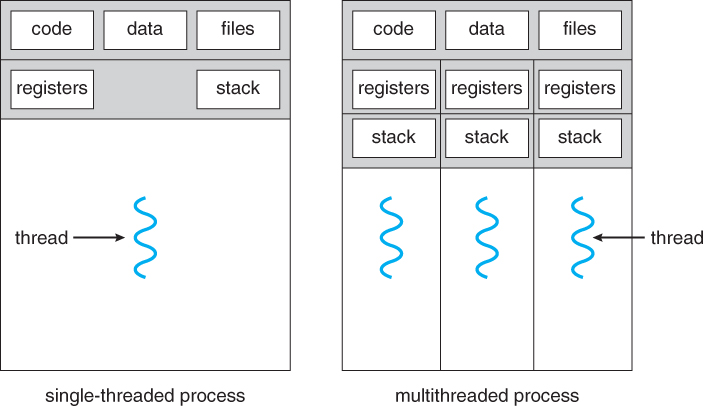
\includegraphics[scale=0.85]{./Drawings/EDAF35-Operating_Systems/ThreadDiagram.jpg}
  \caption{Single- vs. Multithread Diagram}
  \label{fig:Thread_Diagram}
\end{figure}

The biggest benefits of using multiple \nameref{def:Thread}s are:
\begin{enumerate}[noitemsep]
\item \textbf{Responsiveness}.
  Multithreading an interactive application may allow a program to continue running even if part of it is blocked or is performing a lengthy operation, thereby increasing responsiveness to the user.
  This quality is especially useful in designing user interfaces.
\item \textbf{Resource sharing}.
  \nameref{def:Process}es can only share resources through techniques such as \nameref{par:Message_Passing} and \nameref{par:Message_Passing}.
  Using these techniques requires explicit arrangement by the programmer.
  However, threads share the memory and the resources of the process to which they belong, allowing an application to have several different threads of activity within the same address space.
\item \textbf{Economy}.
  Allocating memory and resources for process creation is costly.
  Because threads share the resources of the process to which they belong, it is more economical to create and context-switch threads.
\item \textbf{Scalability}.
  The benefits of multithreading can be even greater in a multiprocessor architecture, where threads may be running in parallel on different processing cores.
  A single-threaded process can run on only one processor, regardless how many are available.
\end{enumerate}

\begin{definition}[Parallelism]\label{def:Parallelism}
  \emph{Parallelism} is where a system can perform more than one task simultaneously.
\end{definition}

\begin{definition}[Concurrency]\label{def:Concurrency}
  \emph{Concurrency} supports more than one task executing simulataneiously, and allows all the tasks to make progress.
  Thus, it is possible to have concurrency without \nameref{def:Parallelism}.
\end{definition}

To handle the increase in \nameref{def:Process} \nameref{def:Thread} counts, many CPUs support more than one thread per core.
This means multiple threads can be loaded into the CPU for faster switching.
On desktop Intel CPUs, this is called \textbf{hyperthreading}.

The biggest difficulties in using multiple \nameref{def:Thread}s are:
\begin{enumerate}[noitemsep]
\item \textbf{Identifying tasks}.
  Examine applications to find areas that can be divided into independent tasks that can be run concurrently on individual cores.
\item \textbf{Balance}.
  While identifying tasks that can run in parallel, programmers must also ensure that the tasks perform equal work of equal value.
  In some instances, a certain task may not contribute as much value to the overall process as other tasks.
\item \textbf{Data splitting}.
  Just as applications are divided into separate tasks, the data accessed and manipulated by the tasks must be divided to run on separate cores.
\item \textbf{Data dependency}.
  The data accessed by the tasks must be examined for dependencies between two or more tasks.
  When one task depends on data from another, the tasks must be synchronized to accommodate the data dependency.
\item \textbf{Testing and debugging}.
  When a program is running in parallel on multiple cores, many different execution paths are possible, making testing and debugging much harder.
\end{enumerate}

There are 2 distinct types of \nameref{def:Parallelism}, though many applications use both of them.
\begin{enumerate}[noitemsep]
\item \nameref{def:Data_Parallelism}
\item \nameref{def:Task_Parallelism}
\end{enumerate}

\begin{definition}[Data Parallelism]\label{def:Data_Parallelism}
  \emph{Data parallelism} focuses on distributing subsets of the same data across multiple computing cores and performing the same operation on each core.
  For example, summing the contents of an array of size $N$.
  On a single-core system, one thread would simply sum the elements $[0] \ldots [N-1]$.
  On a dual-core system, however, thread A, running on core 0, could sum the elements $[0] \ldots [\frac{N}{2}-1]$ while thread B, running on core 1, could sum the rest of the elements $[\frac{N}{2}] \ldots [N-1]$.
\end{definition}

\begin{definition}[Task Parallelism]\label{def:Task_Parallelism}
  \emph{Task parallelism} involves distributing tasks/\nameref{def:Thread}s across multiple computing cores.
  Each thread is performing a unique operation.
  Different threads may be operating on the same data, or they may be operating on different data.
\end{definition}

\subsection{User and Kernel Threads}\label{subsec:User_Kernel_Threads}
A relationship must exist between \nameref{def:User_Thread}s and \nameref{def:Kernel_Thread}s.
There are three common ways of establishing such a relationship:
\begin{enumerate}[noitemsep]
\item The \nameref{subsubsec:Many_To_One_Model}
\item The \nameref{subsubsec:One_To_One_Model}
\item The \nameref{subsubsec:Many_To_Many_Model}
\end{enumerate}

\begin{definition}[User Thread]\label{def:User_Thread}
  \emph{User thread}s are \nameref{def:Thread}s created by a \nameref{def:User} \nameref{def:Process}.
  They are supported above the kernel and are managed without kernel support.
\end{definition}

\begin{definition}[Kernel Thread]\label{def:Kernel_Thread}
  \emph{Kernel thread}s are \nameref{def:Thread}s created by the \nameref{def:Kernel}.
  They are supported and managed directly by the operating system.
\end{definition}

\subsubsection{Many-To-One Model}\label{subsubsec:Many_To_One_Model}
\textbf{This model maps many user-level threads to a single \nameref{def:Kernel_Thread}.}
Thread management is done by the thread library in user space, so it is efficient.
However, the entire process will block if a thread makes a blocking system call.
Also, because only one thread can access the kernel at a time, multiple threads are unable to run in parallel on multicore systems.

\subsubsection{One-To-One Model}\label{subsubsec:One_To_One_Model}
\textbf{This model maps each user thread to an individual kernel thread.}
It provides more concurrency than the many-to-one model by allowing another thread to run when a thread makes a blocking system call.
It also allows multiple threads to run in parallel on multiprocessors.

The only drawback to this model is that creating a user thread requires creating the corresponding kernel thread, which is quite expensive.
The overhead of creating kernel threads can hurt the performance of an application.
To combat this, most implementations of this model restrict the number of threads supported by the system.
Most desktop operating systems use this model.

\subsubsection{Many-To-Many Model}\label{subsubsec:Many_To_Many_Model}

%%% Local Variables:
%%% mode: latex
%%% TeX-master: "../../EDAF35-Operating_Systems-Reference_Sheet"
%%% End:


\subsection{Thread Libraries}\label{subsec:Thread_Libraries}
\begin{definition}[Thread Library]\label{def:Thread_Library}
  A \emph{thread library} is an \nameref{def:API} that allows a programmer to create and manage \nameref{def:Thread}s.
\end{definition}

There are 2 main ways to implement a \nameref{def:Thread_Library}:
\begin{enumerate}[noitemsep]
\item Provide a library entirely in user space with no kernel support.
  All code and data structures for the library exist in \textbf{user-space}.
  This means that invoking a library function results in a function call in user space and not a system call.
\item Implement a kernel-level library supported directly by the operating system.
  All code and data structures for the library exist in \textbf{kernel-space}.
  Invoking a library function results in a \nameref{def:System_Call} to the \nameref{def:Kernel}.
\end{enumerate}

There are 3 different libraries that are used frequently.
\begin{enumerate}[noitemsep]
\item POSIX Pthreads.
  \begin{itemize}[noitemsep]
  \item This provides a standard interface for \textbf{how the threads should behave}.
  \item The actual implementation details are left for the implementor to decide.
  \item Global variables are shared between threads.
  \item Brought in by the standard library's \kernelinline{pthread.h} header.
  \end{itemize}
\item Windows' Threads.
  \begin{itemize}[noitemsep]
  \item Global variables are shared between threads.
  \item Must include the \kernelinline{windows.h} header.
  \end{itemize}
\item Java's Threads.
\end{enumerate}


%%% Local Variables:
%%% mode: latex
%%% TeX-master: "../../EDAF35-Operating_Systems-Reference_Sheet"
%%% End:


\subsection{Implicit Threading}\label{subsec:Implicit_Threading}
Because programs are starting to use so many \nameref{def:Thread}s that it is becoming hard to manage, the creation and management of threads is moving from developers to compilers/run-time libaries.
This way, the computer manages threads rather than the programmer.

\begin{definition}[Implicit Threading]\label{def:Implicit_Threading}
  \emph{Implicit Threading} is the transfer of \nameref{def:Thread} creation and management away from the programmer, and to the compiler and/or run-time libaries.
  This frees the programmer from having to think/worry about the issues that arise because of multithreading, while still allowing programs to take advantage of the benefits of multithreading.
\end{definition}

There exist 3 main methods for implementing implicit threading:
\begin{enumerate}[noitemsep]
\item \nameref{subsubsec:Thread_Pools}
\item \nameref{subsubsec:OpenMP}
\item \nameref{subsubsec:Grand_Central_Dispatch}
\end{enumerate}

\subsubsection{Thread Pools}\label{subsubsec:Thread_Pools}
\subsubsection{OpenMP}\label{subsubsec:OpenMP}
\subsubsection{Grand Central Dispatch}\label{subsubsec:Grand_Central_Dispatch}
%%% Local Variables:
%%% mode: latex
%%% TeX-master: "../../EDAF35-Operating_Systems-Reference_Sheet"
%%% End:


\subsection{Threading Issues}\label{subsec:Threading_Issues}
In this section, we will discuss some common issues that arise because of multithreading.

\subsubsection{The \texorpdfstring{\kernelinline{fork()}}{\texttt{fork()}} and \texorpdfstring{\kernelinline{exec()}}{\texttt{exec()}} System Calls}\label{subsubsec:Fork_Exec_System_Calls}
Since \kernelinline{fork()} creates a separate, but duplicate, child \nameref{def:Process} from its parent, what are the semantics when creating a \nameref{def:Thread} on a UNIX system, since \nameref{def:Thread}s are just another kind of \nameref{def:Process}?

If one thread in a program calls \kernelinline{fork()}, does the new process duplicate all threads, or is the new process single-threaded?
To answer this, there are two versions of \kernelinline{fork()}, one that duplicates all threads and another that duplicates only the thread that invoked the \kernelinline{fork()} system call.

The \kernelinline{exec()} system call is relatively unchanged; if a thread invokes the \kernelinline{exec()} system call, the program specified in the parameter to \kernelinline{exec()} will \textbf{replace the entire process}, including all threads.

Which version of \kernelinline{fork()} to use depends on the application.
If \kernelinline{exec()} will be called immediately after forking, then duplicating \textbf{all} threads is unnecessary, as the program specified in the parameters to \kernelinline{exec()} will replace the process anyways, thus duplicating only the calling thread is appropriate.
If, however, the separate process does not call \kernelinline{exec()} after forking, the separate process should duplicate all threads.

\subsubsection{Signal Handling}\label{subsubsec:Signal_Handling}
\begin{definition}[Signal]\label{def:Signal}
  A UNIX \emph{signal} is used to notify a \nameref{def:Process} that an event has occurred.
  The reception of the signal can be synchronous or asynchronous.
  Synchronous in this context means that the signal is \textbf{delivered to the same proces that caused the signal}.
  Asynchronous means the signal is generated by an event \textbf{external to the running process}, such as keyboard presses or timer expiration.

  Which one depends on the source of and the reason for the event to be signaled.
  However, all signals have the same general pattern:
  \begin{enumerate}[noitemsep]
  \item A signal is generated by the occurrence of a particular event.
  \item The signal is delivered to a process.
  \item Once delivered, the signal must be handled.
  \end{enumerate}
\end{definition}

When a \nameref{def:Signal} is delivered, it must be handled by either:
\begin{enumerate}[noitemsep]
\item The default signal handler
\item The user-defined signal handler
\end{enumerate}


%%% Local Variables:
%%% mode: latex
%%% TeX-master: "../../EDAF35-Operating_Systems-Reference_Sheet"
%%% End:


\subsection{Linux Implementation of Threads}\label{subsec:Linux_Implementation_Threads}
\nameref{def:Thread}s are a popular modern programming abstraction.
They provide multiple executors within the same program in a shared memory address space.
They can also share open files and other resources.
\nameref{def:Thread}s enable concurrent programming and, on multiple processor systems, true parallelism.

The Linux kernel is unique in that there is no concept of a \nameref{def:Thread}.
Instead, Linux implements all \nameref{def:Thread}s as standard \nameref{def:Process}es.
The Linux kernel does not provide any special scheduling semantics or data structures to represent \nameref{def:Thread}s.
Instead, a \nameref{def:Thread} is merely a \nameref{def:Process} that shares certain resources with other \nameref{def:Process}es.
Each \nameref{def:Thread} has a unique \kernelinline{task_struct} and appears to the kernel as a normal \nameref{def:Process} which just happen to share resources, such as an address space, with other \nameref{def:Process}es.

For example, assume you have a \nameref{def:Process} that consists of four \nameref{def:Thread}s.
In Linux, there are simply four \nameref{def:Process}es and thus four normal \kernelinline{task_struct} structures.
The four \nameref{def:Process}es are set up to share certain resources.
The result is quite elegant.
However, on systems with explicit \nameref{def:Thread} support, one \nameref{def:Process_Descriptor} might exist that points to the four different \nameref{def:Thread}s.
The \nameref{def:Process_Descriptor} describes the shared resources, such as an address space or open files.
The \nameref{def:Thread}s then describe the resources they alone possess.

\subsubsection{Creating Threads}\label{subsubsec:Creating_Threads}
\nameref{def:Thread}s are created the same as normal \nameref{def:Process}es, i.e.\ \kernelinline{fork()} is used.
The difference is that the \kernelinline{clone()} \nameref{def:System_Call} is passed flags corresponding to the specific resources to be shared.
\begin{minted}[frame=lines,linenos]{c}
clone(CLONE_VM | CLONE_FS | CLONE_FILES | CLONE_SIGHAND, 0);
\end{minted}

The code above results in behavior identical to a normal \kernelinline{fork()}, except that the address space, filesystem resources, file descriptors, and signal handlers are shared.
In other words, the new task and its parent are what are popularly called \nameref{def:Thread}s.

The flags provided to \kernelinline{clone()} help specify the behavior of the new process and detail what resources the parent and child will share.
\Cref{tab:Clone_Flags} lists the \kernelinline{clone()} flags, which are defined in \kernelinline{<linux/sched.h>}, and their effect.

\begin{table}[h!tbp]
  \centering
  \begin{tabular}{ll}
    \toprule
    \textbf{Flag} & \textbf{Meaning} \\
    \midrule
    \kernelinline{CLONE_FILES} & Parent and child share open files. \\
    \kernelinline{CLONE_FS} & Parent and child share filesystem information. \\
    \kernelinline{CLONE_IDLETASK} & Set PID to zero (used only by the idle tasks). \\
    \kernelinline{CLONE_NEWNS} & Create a new namespace for the child. \\
    \kernelinline{CLONE_PARENT} & Child is to have same parent as its parent. \\
    \kernelinline{CLONE_PTRACE} & Continue tracing child. \\
    \kernelinline{CLONE_SETTID} & Write the TID back to user-space. \\
    \kernelinline{CLONE_SETTLS} & Create a new TLS for the child. \\
    \kernelinline{CLONE_SIGHAND} & Parent and child share signal handlers and blocked signals. \\
    \kernelinline{CLONE_SYSVSEM} & Parent and child share SystemV \texttt{SEM\_UNDO} semantics. \\
    \kernelinline{CLONE_THREAD} & Parent and child are in the same thread group. \\
    \kernelinline{CLONE_VFORK} & \kernelinline{vfork()} was used and the parent will sleep until the child wakes it. \\
    \kernelinline{CLONE_UNTRACED} & Do not let the tracing process force \kernelinline{CLONE_PTRACE} on the child. \\
    \kernelinline{CLONE_STOP} & Start process in the \kernelinline{TASK_STOPPED} state. \\
    \kernelinline{CLONE_SETTLS} & Create a new TLS (thread-local storage) for the child. \\
    \kernelinline{CLONE_CHILD_CLEARTID} & Clear the TID in the child. \\
    \kernelinline{CLONE_CHILD_SETTID} & Set the TID in the child. \\
    \kernelinline{CLONE_PARENT_SETTID} & Set the TID in the parent. \\
    \kernelinline{CLONE_VM} & Parent and child share address space. \\
    \bottomrule
  \end{tabular}
  \caption{\kernelinline{clone()} Flags}
  \label{tab:Clone_Flags}
\end{table}

\subsubsection{Kernel Threads}\label{subsubsec:Kernel_Threads}
It is often useful for the kernel to perform some operations in the background.
The kernel accomplishes this via kernel threads, standard processes that exist solely in kernel-space.

\defKernelThread*{}

Linux delegates several tasks to kernel threads, most notably the \texttt{flush} tasks and the \texttt{ksoftirqd} task.
Kernel threads are created on system boot by other kernel threads.
The kernel handles this automatically by forking all new kernel threads off of the \texttt{kthreadd} \nameref{def:Kernel} process.
The interface for \nameref{def:Kernel_Thread}s is declared in \kernelinline{<linux/kthread.h>}.

When started, a \nameref{def:Kernel_Thread} continues to exist until it calls \kernelinline{do_exit()} or another part of the kernel calls \kernelinline{kthread_stop()}, passing in the address of the \kernelinline{task_struct} structure returned by \kernelinline{kthread_create()}.

%%% Local Variables:
%%% mode: latex
%%% TeX-master: "../../EDAF35-Operating_Systems-Reference_Sheet"
%%% End:


%%% Local Variables:
%%% mode: latex
%%% TeX-master: "../EDAF35-Operating_Systems-Reference_Sheet"
%%% End:
